\chapter{Introduction}
\pagenumbering{alph}
\pagenumbering{arabic}
\pagestyle{plain}
Particle physics is an established branch of physics with a rich history in theory and experiments ever since the beginning of the $20^{\mathrm{th}}$ century. So far the experimental and theoretical research have shown us hand in hand that the universe consists of particles and interaction carriers. Particles of matter, or elementary particles, are divided in two groups -- quarks and leptons. The quarks that we know today are called $u$ (up), $d$ (down), $s$ (strange), $c$ (charm), $b$ (bottom) and $t$ (top). Leptons are further split in charged leptons; $e$ (electron), $\mu$ (muon), $\tau$ (tau lepton), and their corresponding neutrinos; $\nu_e$ (electron neutrino), $\nu_\mu$ (muon neutrino) and $\nu_\tau$ (tau neutrino). Interaction carriers are known as gauge bosons and they are $\gamma$ (photon), $g$ (gluon), $W^\pm$ (charged weak bosons) and $Z^0$ (neutral weak boson). Theoretical calculations also predicted the recently discovered Higgs boson ($H$), which is responsible for the mass of all particles. Some of the particles above also have mirrored versions of themselves, called antiparticles, which exhibit somewhat different properties compared to their un-mirrored versions.

Combinations of quarks such as $q_1 q_2 q_3$ (hadrons) or $q_1 \bar{q}_2$ (mesons) make up heavier particles. Examples of such particles are not only protons and neutrons, but also heavier particles which can be produced in processes involving high enough energies. Such heavy particles are unstable and decay into lighter ones. Together with the elementary particles and interaction carriers, three out of four of these interactions are joined in a theoretical model called the Standard Model (SM) \cite{GLASHOW1961579, PhysRevLett.19.1264, salam1994weak, GIMmech} (see Figure \ref{fig:sm}). Standard Model describes the electromagnetic, weak nuclear and strong nuclear interaction. General relativity -- the theory of gravity -- is not included in the Standard Model, since the two are incompatible on a mathematical level. However, due to its low coupling constant, gravity does not play a significant role in the world of subatomic particles. Experimental studies of particle processes give an insight into the mechanisms of basic interactions between them. By doing so we are able to learn the secrets of the universe and how it all began.


\begin{figure}[H]
	\centering
	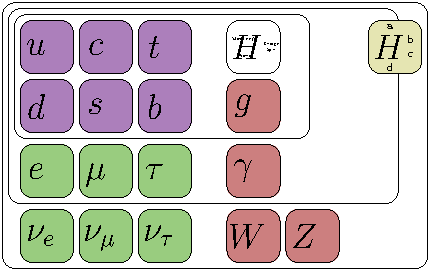
\includegraphics[scale=1.6]{texfig/SM}
	\captionsetup{width=.8\linewidth}
	\caption{A schematic representation of particles in the Standard Model.}
	\label{fig:sm}
\end{figure}

This analysis revolves around decays of the so-called $B$ mesons, which are particles consisting of a $b$ quark and a light $u$ or a $d$ quark. The charged $B^+$ and the neutral $B^0$ meson have a structure of $(\bar b, u)$ and $(\bar b, d)$, respectively, while the antiparticle $B$ mesons are $B^-(b, \bar u)$ and $\bar B{}^0(b, \bar d)$.  Perhaps one of the most surprising features of nature that can be studied with decays of $B$ mesons is the $CP$ symmetry violation ($\cancel{CP}$). $CP$ symmetry is a combination of the $C$ symmetry (charge conjugation) and the $P$ symmetry (spatial inversion). A conservation of the $CP$ symmetry would mean that the mirrored processes, in which all particles are exchanged by the corresponding anti-particles, proceed in exactly the same manner as the original processes. Today we know that this does not hold true for all cases and we, in fact, find processes which violate the $CP$ symmetry. We also know that $\cancel{CP}$ is related to the weak nuclear interaction. Here lies our motivation for studying decays of $B$ mesons, since they exhibit a rich spectrum of decays which proceed via the weak nuclear interaction.

One of the most important properties of the weak interaction is that it can change the flavor of particles. Such processes are forbidden for the electromagnetic and the strong nuclear interaction, but not for the weak one. Information about the quark transition probabilities is merged into a form of a complex matrix called the Cabibbo-Kobayashi-Maskawa (CKM) matrix \cite{cabibbo1963unitary,kobayashi1973cp}
\begin{equation}
V_{CKM} = \begin{bmatrix}
V_{ud} & V_{us} & V_{ub}\\
V_{cd} & V_{cs} & V_{cb}\\
V_{td} & V_{ts} & V_{tb}
\end{bmatrix}.
\end{equation}

The CKM matrix is a unitary matrix and has only four parameters which are free parameters of the theory and hence must be experimentally determined. The unitarity of the CKM matrix provides us with several mathematical identities, out of which the most relevant one for $B$ meson physics is  
\begin{equation}
V_{ud}V_{ub}^* + V_{cd}V_{cb}^* + V_{td}V_{tb}^* = 0.
\end{equation}

It can be represented by a triangle in the complex plane, called the unitarity triangle, shown in Figure~\ref{ut}. The sides and the angles of the unitarity triangle are related to the free parameters of the CKM matrix. All measurements of weak interaction processes involving $B$ mesons depend on the four free parameters of the CKM matrix. Results of such measurements hence determine the sides and angles of the unitarity triangle. The goal is to then combine all such measurements and overconstrain the sides and angles of the unitarity triangle to check if all the sides meet. By improving such measurements one can check whether the SM is consistent, or if there are some contributing physics processes that we do not yet understand. Such processes are commonly referred to as "new physics" (NP). The measurements of the sides and angles of the triangle are done using different decays, with the most important input from $B$ meson decays. This fact represents another motivation to study the B meson decays.

\begin{figure}[H]
	\centering
	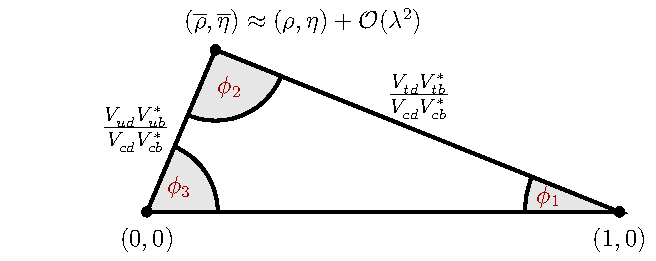
\includegraphics[scale=1]{texfig/UT_Triangle}
	\captionsetup{width=.8\linewidth}
	\caption{The unitarity triangle in the Wolfenstein parametrization \cite{PhysRevLett.51.1945}.}
	\label{ut}
\end{figure}

In this analysis, we focus on the $V_{ub}$ CKM matrix element, which corresponds to $b \to u$ quark transitions. It has the smallest absolute value of all the CKM matrix elements and is currently determined with the largest uncertainty. Such quark transitions are present in charmless semileptonic $B$ meson decays of the form
\begin{equation}
B^+ \to X_u^0 \ell^+ \nu_\ell,
\end{equation}

where $X_u^0$ represents a charmless hadron with a $u$ quark, and $\ell$ is one of the charged leptons, $e,~\mu$ or $\tau$. Measuring the decay rate of the $B$ meson in such decays paves the way for the CKM matrix element determination. Decay rates are directly connected to the $V_{ub}$ element as
\begin{equation}
\mathrm{d} \Gamma \propto G_F^2 \vert V_{ub} \vert ^2 \vert L^\mu \langle X_u \vert \bar u \gamma_u \frac{1}{2} (1-\gamma_5) b \vert B \rangle \vert ^2,
\end{equation}

where $\Gamma$ is the decay width, $G_F$ is the Fermi coupling constant, $L^\mu$ is the leptonic current and the expression in the Dirac brackets is the hadronic current. The factor $\vert V_{ub} \vert ^2$ is the CKM element describing the $b \to u$ quark transition. Measurement of the $V_{ub}$ CKM matrix element can be performed using two general approaches, with the exclusive or inclusive method, which are described below. Both methods require an application of different experimental and theoretical techniques, so they provide largely independent determinations of $\vert V_{ub} \vert$. Currently, both methods also have comparable accuracies. 

In the exclusive method, one studies the decays of $B$ mesons to a specific charmless hadronic final state, such as $B \to \pi \ell \nu$. Clean determination of the $\vert V_{ub}\vert$ is possible due to precise experimental measurements along with reliable theoretical calculations. However, theoretical calculations are more challenging for decays to a specific final state, since hadronization of quarks has to be taken into account. There are also two main experimental challenges in this method. One has to reduce the abundant background from $B \to X_c \ell \nu$ processes since the $b \to c$ quark transition is much more probable than the $b \to u$ transition. The second experimental challenge is to separate $B$ meson decays into a specific charmless hadronic final state from other $B \to X_u \ell \nu$ decays since they populate roughly the same regions of the phase-space as the signal decay.

In the inclusive method, one studies the decays of $B$ mesons to any charmless hadronic final state $B \to X_u \ell \nu$. In this case, the total decay rate for $b \to u \ell \nu$ can be calculated accurately since hadronization does not have to be taken into account. The greater challenge with this method is again the experimental measurement of the total decay rate due to the $B \to X_c \ell \nu$ background. Experimental sensitivity to $V_{ub}$ is highest where $B \to X_c \ell \nu$ decays are less dominant. Theory and experiment have to compromise and limit the $\vert V_{ub}\vert $ determination to a region of phase-space where the signal-to-background ratio is good. Theoretical calculations take this into account by calculating the partial decay rate $\Delta \Gamma$, which is more challenging to determine than the total decay rate. One possible and often used approach to reduce $b \to c$ background is to reject all events with kaons present in the final particle selection. The procedure is called a $K$-veto. Kaons consist of an $s$ quark, which is mainly produced in the dominant $b \to c \to s$ transition chain. This means that if a kaon is found in an event, it is very likely that it originates from a particle with a $c$ quark, indicating the $b \to c$ process. 

If $\vert V_{ub} \vert$ is determined with both of these methods, the values can be compared and potentially combined. It turns out that the consistency between the two results is only marginal, the difference is at a level of $3\sigma$. The current world averages \cite{Amhis:2016xyh} of the exclusive (from $B^0 \to \pi^- \ell^+ \nu$) and inclusive (GGOU collab. \cite{Gambino:2007rp}) methods are
\begin{align}
&\vert V_{ub} \vert_{\mathrm{excl.}} = \left(3.65 \pm 0.09 \pm 0.11\right)\E{-3},\\
&\vert V_{ub} \vert_{\mathrm{incl.}}^{\mathrm{GGOU}} = \left(4.52 \pm 0.15~{}^{+0.11}_{-0.14}\right)\E{-3},
\end{align}
where the first and the second uncertainties are the experimental and the theoretical, respectively. We see that inclusive measurements prefer higher values than exclusive ones. This is known as the $V_{ub}$ puzzle. It is necessary to make further research as to why this difference occurs. The reason could be an unknown experimental or theoretical error, or it is even possible that some NP contributions occur. This analysis will focus on a possible reason that could be hidden in the selection mentioned before. By performing a $K$-veto, one discards all events with kaons in the final state in order to suppress $b \to c$ contributions. We focus on the charged \decaya~decay, which is very similar to the $B \to \pi \ell \nu$, except for a production of an $s \bar s$ quark pair, which then combines with final state quarks to form kaons, as shown in Figure~\ref{feynman}. In this case, we have kaons in the final state where the $B$ meson decayed via a $b \to u$ process. Such decays were discarded in previous $\vert V_{ub} \vert$ determinations with the inclusive method, but in principle, they contribute to the result and should be taken into account. The results of this analysis should help us take a step closer towards solving the $V_{ub}$ puzzle. 

\begin{figure}[H]
	\centering
	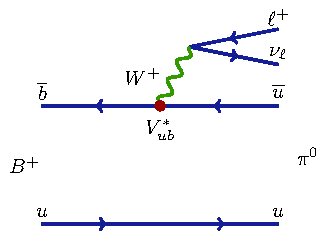
\includegraphics{texfig/B2pilnu}
	\hspace{1cm}
	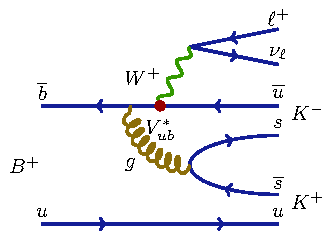
\includegraphics{texfig/B2KKlnu}
	\captionsetup{width=.8\linewidth}
	\caption{Feynman diagrams for the $B^+ \to \pi^0 \ell^+ \nu_\ell$ decay (left) and the $B^+ \to K^- K^+ \ell^+ \nu_\ell$ decay (right).}
	\label{feynman}
\end{figure}

Specifically, we will be focusing on decays of the charged $B$ mesons of the form \decayb, since it includes two charged kaons, as opposed to the case of the neutral $B$ meson decay. The reason for this is a simpler decay chain and a higher reconstruction efficiency. All further occurrences of \decaya~imply decays of the form \decayb~and its charge conjugated counterpart.